\documentclass[UTF8]{report}
\usepackage{graphicx}
\usepackage{xetexko}

\title{%
    <컴퓨터프로그래밍 3> 실습 보고서 \\ 
    \large [제 04 주] 마방진}
\author{201704150 허강준}
\date{\today}


\begin{document}
    \maketitle
    \tableofcontents

    \chapter{프로그램 설명서}
        본 보고서에서는 마방진에 대한 객체를 정의하고 처리하는 프로그램에 대해 기술한다.

        \section{프로그램의 전체 설계 구조 (MVC 등)}
            
            \paragraph{%
                \normalfont 이 프로그램은 마방진 연산을 처리하고 화면에 보여주는 프로그램으로서, 코드 흐름을 \texttt{AppController} 가 제어한다. 마방진 데이터 및 연산을 표현하기 위해 \texttt{MagicSquare} 모델을 생성하였으며 화면에 출력되는 모든 마방진 및 메세지, 입력 안내 등은 \texttt{AppView} 에서 처리한다. 
            }

            
        \section{함수 설명서}

            모델 객체 관련 메서드의 경우 클래스명::메서드명 으로 기술한다. \texttt{static} 메서드의 경우 앞에 \texttt{static}을 붙인다.
            
            \paragraph{\texttt{static MagicSquare::create(int order)}}
            \paragraph{%
                \normalfont 마방진 객체를 생성한다. 인자로 차수 값을 받으며, 객체 생성이 성공할 경우 \texttt{MagicSquare} 의 포인터를 리턴한다.
            }

            \paragraph{\texttt{MagicSquare::destroy()}}
            \paragraph{%
                \normalfont 마방진 객체를 해제한다. 마방진 객체와 내부 마방진 배열은 Heap에 생성된 객체이므로 메모리 누수를 막기 위하여 필수적으로 해제해준다.
            }

            \paragraph{\texttt{static MagicSquare::orderIsValid(int order)}}
            \paragraph{%
                \normalfont 인자로 받은 차수가 마방진에 사용될 수 있는지 검사한다. 경우에 따라 4가지의 정수 값을 리턴한다.
            }

            \begin{itemize}
                \item 0 - 정상
                \item 1 - 너무 큼 (\texttt{MS\_MAX\_ORDER} 보다 큼)
                \item 2 - 너무 작음
                \item 3 - 짝수임
            \end{itemize}

            \paragraph{\texttt{MagicSquare::clear()}}
            \paragraph{%
                \normalfont 현재 마방진 객체의 값을 비운다. (전부 0으로 만든다.)
            }

            \paragraph{\texttt{MagicSquare::solve()}}
            \paragraph{%
                \normalfont 정해진 알고리즘에 따라 마방진 연산을 수행한다.
            }

            \paragraph{\texttt{AppView\_out\_msg\_startMagicSquare(void)}}
            \paragraph{%
                \normalfont \texttt{<<< 마방진 풀이를 시작합니다 >>>} 메세지를 출력한다.
            }

            \paragraph{\texttt{AppView\_out\_msg\_endMagicSquare(void)}}
            \paragraph{%
                \normalfont \texttt{<<< 마방진 풀이를 종료합니다 >>>} 메세지를 출력한다.
            }

            \paragraph{\texttt{AppView\_msg\_allocationFailed(void)}}
            \paragraph{%
                \normalfont \texttt{MagicSquare} 객체의 할당이 실패하였을 때 오류 메세지를 출력한다.
            }

            \paragraph{\texttt{AppView\_out\_printMagicSquare(MagicSquare* ms)}}
            \paragraph{%
                \normalfont 마방진을 출력한다. \texttt{MagicSquare} 객체를 받아 내부의 \texttt{order}에 따라 출력한다.
            }

            \paragraph{\texttt{AppView\_err\_msg\_orderTooSmall(void)}}
            \paragraph{\texttt{AppView\_err\_msg\_orderIsNotOdd(void)}}
            \paragraph{\texttt{AppView\_err\_msg\_orderTooLarge(void)}}
            \paragraph{%
                \normalfont 입력받은 차수가 정상적이지 않을 경우 관련 오류메세지를 출력한다.
            }

            \paragraph{\texttt{AppView\_in\_getNextOrder(void)}}
            \paragraph{%
                \normalfont 정숫값 입력을 사용자로부터 받아 리턴한다.
            }


        \section{종합 설명서}

            \paragraph{%
                \normalfont 마방진은 모든 행과 열, 그리고 대각선의 합이 전부 동일하도록 수를 정사각행렬에 배치한 것이다. 1부터 $n^2$ 까지의 자연수가 차례로 배치된다.첫번째 행의 중앙부터 
            }

            \paragraph{%
                \normalfont 본 프로그램에서는 실습 자료에서 제시된 알고리즘을 사용하였으며 그 방법은 다음과 같다:
            }

            \begin{itemize}
                \item 첫번째 행의 중앙 열 s부터 시작한다. (차수 n에 대해 $s = n >> 1$, >>는 우측 쉬프트 연산)
                \item 오른쪽 위로 올라가며 1씩 증가한다.
                \item 만일 채우고자 하는 칸에 이미 값이 채워진 경우 현재 칸의 바로 아래 칸을 채운다.
                \item 이때 행렬을 벗어날 경우, 다음 규칙에 따라 다음 칸을 선정한다:\\
                      \begin{itemize}
                          \item 위쪽 방향일 경우 마지막 행으로 이동한다.
                          \item 아랫쪽 방향일 경우 처음 행으로 이동한다.
                          \item 오른쪽 방향일 경우 첫 열로 이동한다.
                          \item 왼쪽 방향일 경우 마지막 열로 이동한다.
                      \end{itemize}
            \end{itemize}

            \paragraph{%
                \normalfont 이번 주 과제부터 실험적으로 OOP/MVC Framework를 작성하여 적용하였다. C는 언어적 차원에서 OOP 지원이 타 언어에 비해 미비하므로 각종 Boilerplate에 대한 매크로를 작성하여 더욱 편리하게 OOP 코드를 작성할 수 있다.
            }
            
    \chapter{프로그램 장단점/특이점 분석}
        \section{OOP/MVC 프레임워크 분석}
            \paragraph{%\
                \normalfont C는 본래 절차지향 컨셉트의 언어로, 객체지향에 대한 지원이 다른 언어에 비해 미비하다. 구조체를 이용할 수도 있으나 C의 구조체는 근본적으로 함수 자체를 포함할 수 없다. (함수 포인터는 함수가 아니다.)
            }

            \paragraph{%\
                \normalfont 따라서 이번 강의 내내 C에 쓰기 적합한 형태의 매크로/Boilerplate 등을 제공하는 OOP 프레임워크를 구상하고 있으며 이번 과제부터 계속 적용될 예정이다.
            }

            \paragraph{%\
                \normalfont 우선, \texttt{CLASS}는 \texttt{typedef struct \{\} class\_name}의 매크로로, \texttt{typedef struct}등의 반복 타이핑을 지양하고 좀 더 시맨틱하게 접근 가능하게끔 구상되었다.
            }

            \paragraph{%\
                \normalfont 대부분의 객체지향 프로그래밍 언어들은 자기 자신을 지칭하는 예약어를 언어 스펙에서 제공한다. C++/Java의 \texttt{this} 가 그 경우이며 이 외에도 \texttt{self}(Javascript, Python), \texttt{Me}(Visual Basic) 등이 있다.
            }
        
            \paragraph{%\
                \normalfont 따라서 가독성을 해치지 않는 선에서 이러한 키워드를 최대한 자연스럽게 제공하고자 하였으며 그 결과 함수 선언시 첫번째 인자로 \texttt{self} 라는 이름을 가진 포인터를 정의하도록 하는 매크로 \texttt{METHOD\_DEF} 를 사용하였다. 해당 매크로로 정의된 메서드는 다시 \texttt{METHOD} 라는 매크로로 호출 가능하다.
            }

            \paragraph{%\
                \normalfont 반면 \texttt{self}를 사용할 수 없는 정적 메서드 또한 지원할 필요가 있었는데, 이 경우 \texttt{METHOD\_STATIC\_DEF}를 이용하여 정의할 수 있다. 위에서 서술한 \texttt{METHOD\_DEF}는 내부적으로 \texttt{METHOD\_STATIC\_DEF}를 호출하는 형태로 수행된다.
            }

            \paragraph{%\
                \normalfont 이 외에도 접근 지정자, 생성자, 소멸자 등 여러 객체지향의 컨셉트들을 적용하고자 노력중이며 현재로서는 상술한 형태가 전부이다.
            }

        \section{AppView에 대해 적용하지 않은 이유}    
            \paragraph{%\
                \normalfont 앞서 4주차 2차방정식 프로그램에서 \texttt{AppView} 관련 함수들에 대해서 전부 AppView라는 정적 메서드로 보고 \texttt{METHOD\_STATIC\_DEF}를 이용하여 정의하였으나 이는 불필요한 키워드 반복으로 인한 코드 가독성 저하 및 유지보수를 어렵게 하는 요인이 되었다.
            }

            \paragraph{%\
                \normalfont 따라서 이 과제에서만 일시적으로 원래 C 문법으로 복귀하였으며 좀 더 적합한 형태의 매크로가 있을 지에 대해 연구할 예정이다.
            }
    \chapter{실행 결과 분석}
        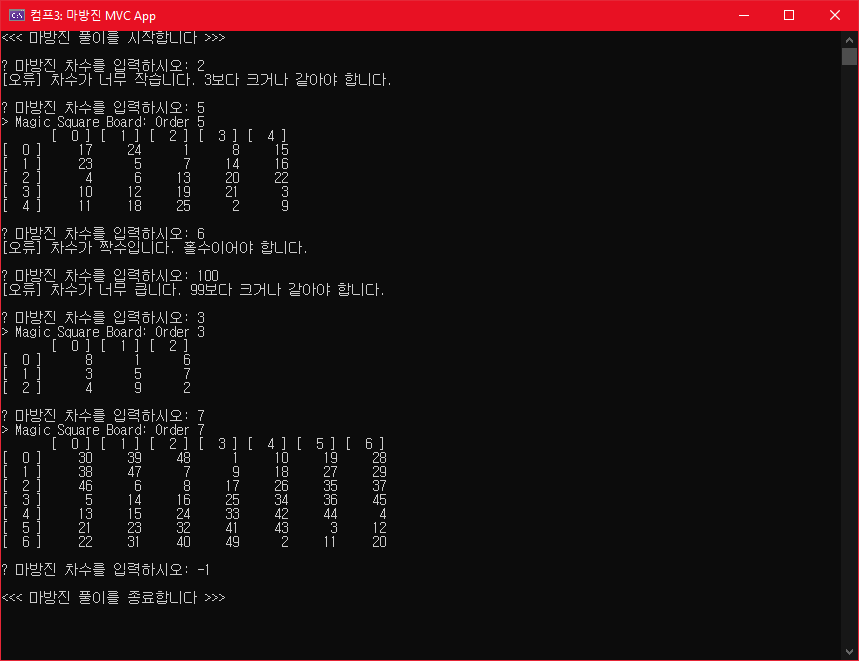
\includegraphics[width=\textwidth]{test_result.png}
        \section{입력과 출력}
            실습 자료에서 제시된 입력을 사용하였으며 모든 경우에 대해 정상적으로 처리됨을 확인하였음.
        \section{결과 분석}
            실습 자료에서 제시된 출력과 동일함을 확인하였음.

    \chapter{소스코드}
        소스코드는 제출된 압축파일에 같이 동봉되어있으며 GitHub (0x00000FF/CNUCSE-Computer-Programming-III-2020-Spring) 에서도 열람할 수 있다.
\end{document}